% !Mode:: "TeX:UTF-8"
% !TEX program  = pdflatex
\documentclass[a4paper]{article}

% import settings, modify the number of homework in this file

\usepackage[T1]{fontenc}
\usepackage{amsmath, amssymb, amsthm}
% amsmath: equation*, amssymb: mathbb, amsthm: proof
\usepackage{moreenum}
\usepackage{mathtools}
\usepackage{url}
\usepackage{graphicx}
\usepackage{subcaption}
\usepackage{booktabs} 
\usepackage[mathcal]{eucal}
\usepackage{dsfont}
\usepackage{geometry}
\geometry{left=30mm,right=30mm,	top=42mm, bottom=33mm}

\usepackage[numbered,framed]{matlab-prettifier}
\lstset{
	style              = Matlab-editor,
	captionpos         =b,
	basicstyle         = \mlttfamily,
	escapechar         = ",
	mlshowsectionrules = true,
}

% set the homework count number
\usepackage[thehwcnt = 1]{iidef}

\newcommand\dif{\text{d}}
\newcommand\no{\noindent}
\newcommand\dis{\displaystyle}
\newcommand\ls{\leqslant}
\newcommand\gs{\geqslant}

\newcommand\limit{\dis\lim\limits}
\newcommand\limn{\dis\lim\limits_{n\to\infty}}
\newcommand\limxz{\dis\lim\limits_{x\to0}}
\newcommand\limxi{\dis\lim\limits_{x\to\infty}}
\newcommand\limxpi{\dis\lim\limits_{x\to+\infty}}
\newcommand\limxni{\dis\lim\limits_{x\to-\infty}}
\newcommand\limtpi{\dis\lim\limits_{t\to+\infty}}
\newcommand\limtni{\dis\lim\limits_{t\to-\infty}}

\newcommand\sumn{\dis\sum\limits_{n=1}^{\infty}}
\newcommand\sumnz{\dis\sum\limits_{n=0}^{\infty}}

\newcommand\sumi{\dis\sum\limits_{i=1}^{\infty}}
\newcommand\sumiz{\dis\sum\limits_{i=0}^{\infty}}
\newcommand\sumin{\dis\sum\limits_{i=1}^{n}}
\newcommand\sumizn{\dis\sum\limits_{i=0}^{n}}

\newcommand\sumk{\dis\sum\limits_{k=1}^{\infty}}
\newcommand\sumkz{\dis\sum\limits_{k=0}^{\infty}}
\newcommand\sumkn{\dis\sum\limits_{k=0}^n}
\newcommand\sumkfn{\dis\sum\limits_{k=1}^n}

\newcommand\pzx{\dis\frac{\partial z}{\partial x}}
\newcommand\pzy{\dis\frac{\partial z}{\partial y}}

\newcommand\pfx{\dis\frac{\partial f}{\partial x}}
\newcommand\pfy{\dis\frac{\partial f}{\partial y}}

\newcommand\pzxx{\dis\frac{\partial^2 z}{\partial x^2}}
\newcommand\pzxy{\dis\frac{\partial^2 z}{\partial x\partial y}}
\newcommand\pzyx{\dis\frac{\partial^2 z}{\partial y\partial x}}
\newcommand\pzyy{\dis\frac{\partial^2 z}{\partial y^2}}

\newcommand\pfxx{\dis\frac{\partial^2 f}{\partial x^2}}
\newcommand\pfxy{\dis\frac{\partial^2 f}{\partial x\partial y}}
\newcommand\pfyx{\dis\frac{\partial^2 f}{\partial y\partial x}}
\newcommand\pfyy{\dis\frac{\partial^2 f}{\partial y^2}}

\newcommand\intzi{\dis\int_{0}^{+\infty}}
\newcommand\intd{\dis\int}
\newcommand\intab{\dis\int_a^b}

\newcommand{\degree}{^\circ}

\newcommand\ma{\mathcal{A}}
\newcommand\mb{\mathcal{B}}
\newcommand\mc{\mathcal{C}}
\newcommand\me{\mathcal{E}}
\newcommand\mg{\mathcal{g}}

\newcommand\mcc{\mathbb{C}}
\newcommand\mrr{\mathbb{R}}
\newcommand\mzz{\mathbb{Z}}

\newcommand\mx{\bf{x}}
\newcommand\mX{\bf{X}}
\newcommand\my{\bf{y}}
\newcommand\mY{\bf{Y}}
%%=============================================

%%=====定义新数学符号===============================
\DeclareMathOperator{\sgn}{sgn}
\DeclareMathOperator{\arccot}{arccot}
\DeclareMathOperator{\arccosh}{arccosh}
\DeclareMathOperator{\arcsinh}{arcsinh}
\DeclareMathOperator{\arctanh}{arctanh}
\DeclareMathOperator{\arccoth}{arccoth}
\DeclareMathOperator{\grad}{\bf{grad}}
%\DeclareMathOperator{\argmax}{argmax}
%\DeclareMathOperator{\argmin}{argmin}
%\DeclareMathOperator{\diag}{diag}
\DeclareMathOperator{\csign}{csign}
%===============================================

\thecourseinstitute{Harbin Institute of Technology, ShenZhen}
\thecoursename{Operations Research}
\theterm{Fall 2019}
\hwname{Homework}

\begin{document}
\courseheader
\name{JingXuan Yang, SZ160310217}

\begin{enumerate}
  \setlength{\itemsep}{3\parskip}

% first exercise
  \item The Primo Insurance Company is introducing two new product lines: special risk insurance and mortgages. The expected profit is \$5 per unit on special risk insurance and \$2 per unit on mortgages. Management wishes to establish sales quotas for the new product lines to maximize total expected profit. The work requirements are as follows:
  \begin{figure}[htbp]
  	\centering
  	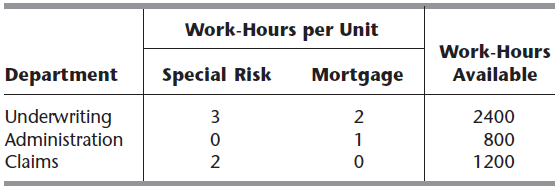
\includegraphics[width = 0.5\textwidth]{fig3-1-9}
  \end{figure}

    \begin{enumerate}
    \item Formulate a linear programming model for this problem.
     \begin{enumerate}
     	\item Decision variables:
     	\begin{equation*}
     	\begin{aligned}
     	x_1&=\text{number of special risk insurances}\\
     	x_2&=\text{number of mortgages}\\
     	\end{aligned}
     	\end{equation*}
     	\item Objective function:
     	\begin{equation*}
     		\max\quad Z=5x_1+2x_2
     	\end{equation*}
     	\item Constraints:
     	\begin{equation*}
     	\begin{aligned}
     	3x_1+2x_2&\ls 2400\\
     	x_2&\ls 800\\
     	2x_1&\ls 1200\\
     	x_1,\ x_2&\gs 0\\
     	\end{aligned}
     	\end{equation*}
     \end{enumerate} 
    \item Use the graphical method to solve this model.
    
    \hspace{2em} First draw the feasible region, which is the shaded area shown in Fig.\ref{gra1}. Then use the slope-intercept form of the objective function to find the optimal solution, which passes through the CPF $(600,300)$.
               \begin{figure}[htbp]
              	\centering
              	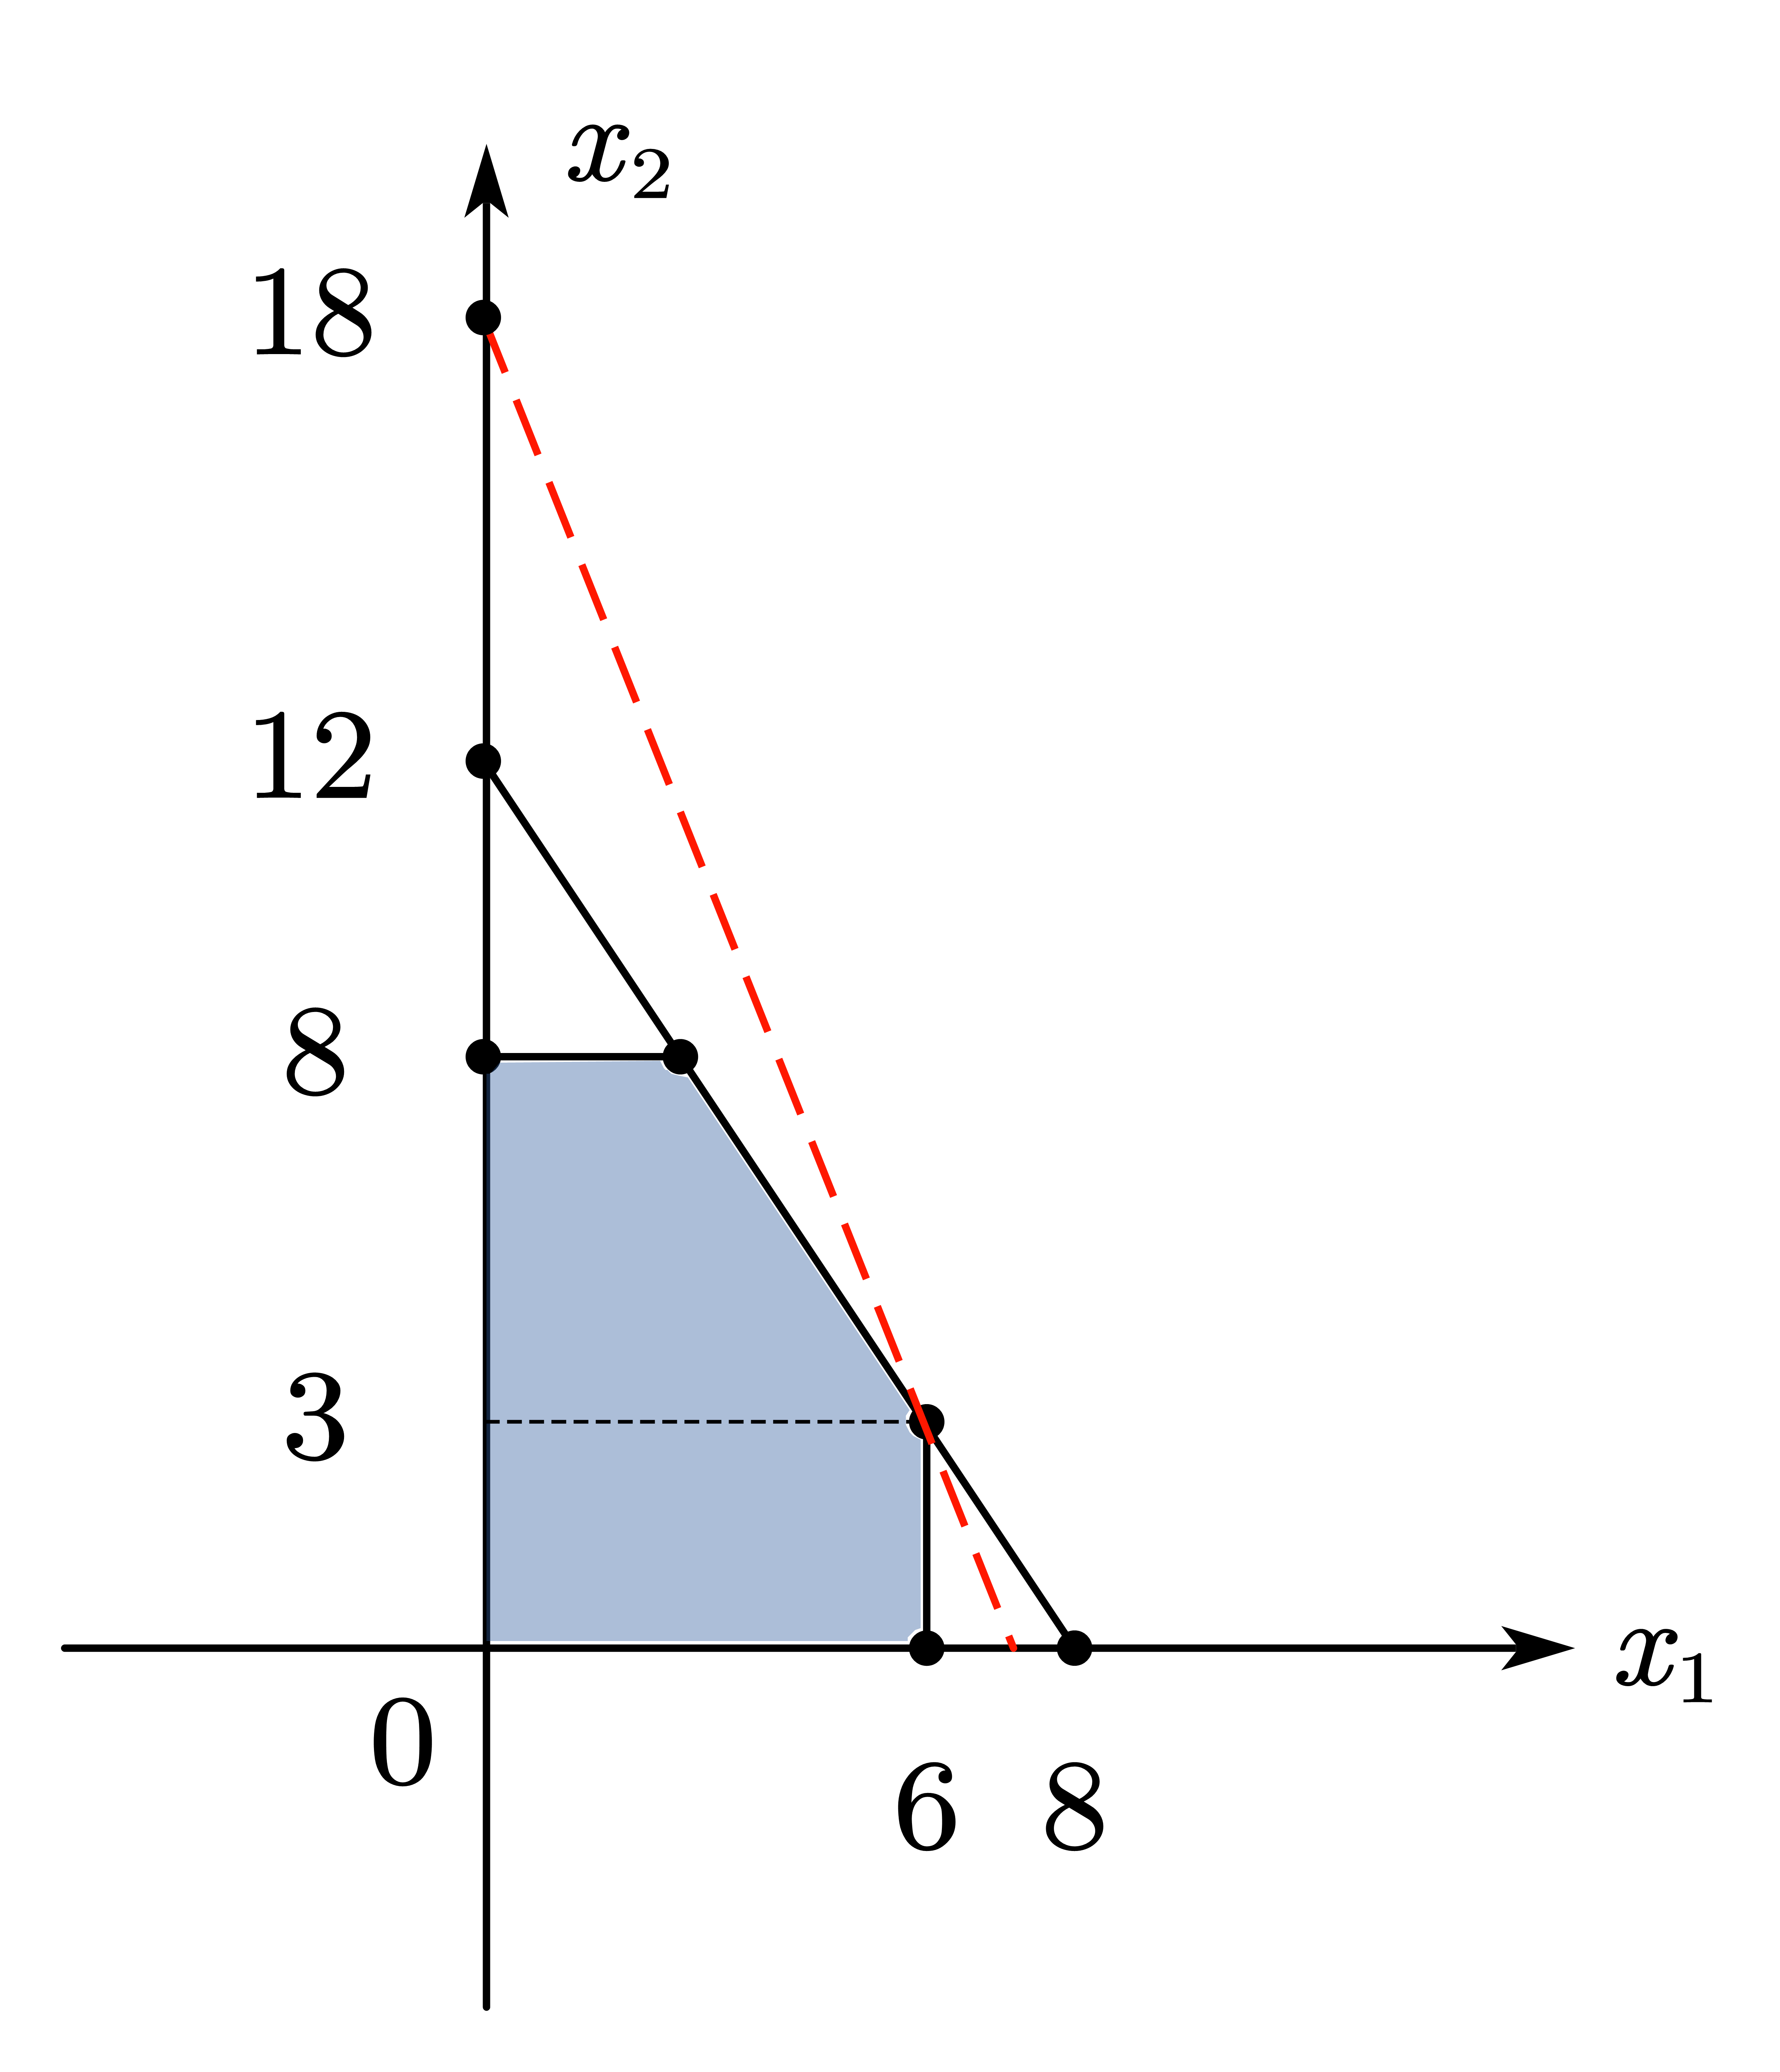
\includegraphics[width = 0.3\textwidth]{graph1}
              	\caption{graphical solution}
              	\label{gra1}
              \end{figure}  
          
          Therefore, the optimal solution is $x_1=600,\ x_2=300$, with $Z=3600$.
    \end{enumerate}

% second excerise
  \item A cargo plane has three compartments for storing cargo: front, center, and back. These compartments have capacity limits on both weight and space, as summarized below:
   \begin{figure}[htbp]
  	\centering
  	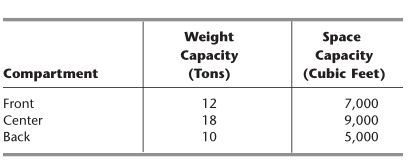
\includegraphics[width = 0.5\textwidth]{fig3-4-14}
  \end{figure}  

Furthermore, the weight of the cargo in the respective compartments must be the same proportion of that compartment's weight capacity to maintain the balance of the airplane. 

\hspace{2em} The following four cargoes have been offered for shipment on an upcoming flight as space is available:
   \begin{figure}[htbp]
	\centering
	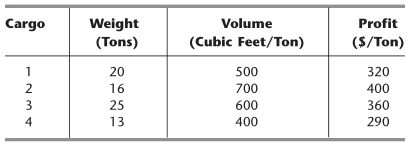
\includegraphics[width = 0.5\textwidth]{fig3-4-14-2}
\end{figure}  

Any portion of these cargoes can be accepted. The objective is to determine how much (if any) of each cargo should be accepted and how to distribute each among the compartments to maximize the total profit for the flight.
\begin{enumerate}
	\item Formulate a linear programming model for this problem.
	\begin{enumerate}
		\item Decision variables:
		
		$x_{ij}:=$ tons of cargo $i$ in compartment $j$, $i=1,2,3,4,\ j=1,2,3$, listed in Tab.\ref{tab1}.
			\begin{table}[h]
				\centering
				\caption{Decision variables}
				\label{tab1}
				\begin{tabular}{cccc}
					\toprule[1.5pt]
					Cargo&Front&Center&Back\\
					\midrule[0.5pt]
					1&$x_{11}$&$x_{12}$&$x_{13}$\\
					2&$x_{21}$&$x_{22}$&$x_{23}$\\
					3&$x_{31}$&$x_{32}$&$x_{33}$\\
					4&$x_{41}$&$x_{42}$&$x_{43}$\\
					\bottomrule[1.5pt]
				\end{tabular}
			\end{table}
		\item Objective function:
		\begin{equation*}
		\max \quad	Z=320\sum_{k=1}^{3}x_{1k}+400\sum_{k=1}^{3}x_{2k}+360\sum_{k=1}^{3}x_{3k}+290\sum_{k=1}^{3}x_{4k}
		\end{equation*}
		\item Constraints:
		
		1. Usable weight in each compartment:
		\begin{equation*}
		\sum_{j=1}^{4}x_{j1}\ls 12,\ \sum_{j=1}^{4}x_{j2}\ls 18,\ \sum_{j=1}^{4}x_{j3}\ls 10
		\end{equation*}
		
		2. Available space in each compartment:
		\begin{equation*}
		\begin{aligned}
		500 x_{11}+700x_{21}+600x_{31}+400x_{41}&\ls 7000\\
		500 x_{12}+700x_{22}+600x_{32}+400x_{42}&\ls 9000\\
		500 x_{13}+700x_{23}+600x_{33}+400x_{43}&\ls 5000\\
		\end{aligned}
		\end{equation*}
		
		3. Total cargoes of each kind:
		\begin{equation*}		
			\sum_{k=1}^{3}x_{1k}\ls 20,\ 
			\sum_{k=1}^{3}x_{2k}\ls 16,\ 
			\sum_{k=1}^{3}x_{3k}\ls 25,\ 
			\sum_{k=1}^{3}x_{4k}\ls 13			
		\end{equation*}
		
		4. Equal weight proportion of cargoes in each compartment:
		\begin{equation*}
		\begin{aligned}
		\dfrac{\sum_{j=1}^{4}x_{j1}}{12}
		=\dfrac{\sum_{j=1}^{4}x_{j2}}{18}
		=\dfrac{\sum_{j=1}^{4}x_{j3}}{10}
		\end{aligned}
		\end{equation*}
		
		5. Nonnegativity:
		\begin{equation*}
		x_{ij}\gs 0,\ i=1,2,3,4,\ j=1,2,3.
		\end{equation*}
	\end{enumerate}
	
\end{enumerate}

% w.r.t the external
\end{enumerate}

%  The source code to plot Figure \ref{fig:1} could be found in Appendix \ref{sec:a:code}. Here are the core codes:
%  \lstinputlisting[firstline=6,lastline=7, firstnumber=6]{matlabscript.m}

%  \newpage
%  \appendix
%  \section{Source code}
%  \label{sec:a:code}
%  % \lstlistoflistings
%  Source code for plotting Figure \ref{fig:1} is shown as follows.
%  \lstinputlisting[caption=FigurePlot]{matlabscript.m}
  
\end{document}
